\documentclass[11pt]{article}

\usepackage{hyperref}
\usepackage{mathtools}
\usepackage{amsthm}
\usepackage{amssymb}
\usepackage{MnSymbol}
\usepackage{mathrsfs}
\usepackage[arrow]{xy}
\usepackage{dsfont}
\usepackage{enumitem}
\usepackage{accents}
\usepackage{tabu}

\pagestyle{headings}

\newcommand{\Z}{\mathbb{Z}}

\theoremstyle{definition}
\newtheorem*{defn}{Definition}

\theoremstyle{definition}
\newtheorem{ex}{Example}

\theoremstyle{plain}
\newtheorem{theo}{Theorem}

\theoremstyle{plain}
\newtheorem*{prop}{Proposition}

\theoremstyle{plain}
\newtheorem{lem}{Lemma}

\theoremstyle{definition}
\newtheorem{que}{Question}

\begin{document}

\author{Stephen Liu}
\title{Thesis Notes}
\date{September 4, 2019}

\maketitle

\subsection*{TODO}
\begin{enumerate}
\item Clean up writing so far.
\end{enumerate}

Outline:
\begin{enumerate}[label=(\alph*)]
\item Introduction to Schroder paths and weightings - primitives for roof and flat step.
\item Explain what $N$ and $D$ are.
\item Taking the second derivative.
\item Simplify $D'/D$ expression immediately.
\item Paths with two flat steps in them. Explain that we only have two big cases (well, three, but by symmetry two).
\item For each case give the additional primitives of M and asymmetric M.
\item mu simplification - identify which cases we now have, but don't need to write out their values explicitly.
\item Give proof that we only need to consider sigma.
\item Then actually simplify sigma and write down what that final expression gives us.
\end{enumerate}

\subsection*{The problem}
Let $d = 2m+1$ where $m$ is a natural number. Denote by $B_2^d$ the $d$-dimensional Euclidean ball and $tB_2^d$ the $d$-dimensional ball with radius $t$ for $t > 0$. In general we are interested in the asymptotic behavior of the magnitude function of the odd dimensional Euclidean ball as we shrink it down to a point. Meckes in \cite{meckes_magnitude_2019} showed that
\begin{equation*}
\frac{d}{dt}\text{Mag}(tB_2^d)\big\vert_{t=0} = \frac{1}{2}V_1(B_2^d)
\end{equation*}
where $V_1(B_2^d)$ is the first instrinsic volume of the Euclidean ball.
We are interested computing the value of
\begin{equation*}
\frac{d^2\text{Mag}(tB_2^d)}{dt^2}\big\vert_{t=0}.
\end{equation*}
We will follow the same approach that Meckes used for the result above, with many of the techniques introduced by Willerton in \cite{willerton_magnitude_2017}.

\subsection*{Explicit magnitude functions for low dimensions}
Barcelo and Carbery in \cite{barcelo_magnitudes_2016} explicitly calculated the magnitude functions of Euclidean balls in dimensions 3,5,7:
\begin{align*}
&\text{Mag}(tB_2^3) = \frac{t^3}{3!}+t^2+2t+1 \\
&\text{Mag}(tB_2^5) = \frac{t^6+18t^5+135t^4+525t^3+1080t^2+1080t+360}{5!(t+3)} \\
&\text{Mag}(tB_2^7) = \frac{t^7}{7!} \\
&+ \frac{\frac{1}{180}t^9+\frac{2}{15}t^8+\frac{3}{2}t^7+\frac{31}{3}t^6+\frac{189}{4}t^5+145t^4+\frac{1165}{4}t^3+360t^2+240t+60}{t^3+12t^2+48t+60}
\end{align*}
So taking second derivatives and evaluating at $t = 0$, we have
\begin{align*}
&\frac{d\text{Mag}^2(tB_2^3)}{dt^2}\big\vert_{t=0} = 2 \\
&\frac{d\text{Mag}^2(tB_2^5)}{dt^2}\big\vert_{t=0} = \frac{38}{9} = 4.222\dots \\
&\frac{d\text{Mag}^2(tB_2^7)}{dt^2}\big\vert_{t=0} = \frac{162}{25} = 6.48 \\
\end{align*}

We will use these values as sanity checks to compare against throughout our calculations.

\subsection*{Schröder paths}
Willerton in \cite{willerton_magnitude_2017} gave an expression for the magnitude function of odd dimensional balls in terms of collections of Schröder paths. We introduce them below:
\begin{defn}
\begin{enumerate}[label=$\bullet$]
\item A \textbf{Schröder path} is a finite directed path in the integer lattice in which each step $(x,y)\in\Z^2$ is either an \textbf{ascent} to $(x+1,y+1)$, a \textbf{descent} $(x-1,y-1)$ or a \textbf{flat step} $(x+2,y)$ (note the advance by \emph{two} spaces in the horizontal direction).
\item Fix $k\geq0$. A \textbf{disjoint k-collection} is a family of Schröder paths from $(-i,i)$ to $(i,i)$ for each $0\leq i\leq k$ such that no node in $\Z^2$ is contained in two of the paths (the paths are disjoint).
\item We denote by $X_k$ the set of all disjoint $k$-collections and by $X_k^j$ the set of disjoint $k$-collections with exactly $j$ flat steps.
\end{enumerate}
\end{defn}

When thinking about what kinds of disjoint $k$-collections we can have in $X_k^j$ for some fixed $j$, it is often useful to think about what a path needs to look like for increasing values of $i$. For example, consider the set $X_k^0$, that is, the set of disjoint $k$-collections with exactly 0 flat steps. At $i = 0$ we have the single dot at $(0,0)$ and at $i = 1$, since we are allowed no flat steps, the only possible path we can have is the path made up of one ascent followed immediately by one descent. Then for $i = 2$, the disjoint condition and the presence of the earlier path at height $i=1$ ensures that the only possible path we can have is the path made up of two ascents followed by two descents. We continue this argument for successive values of $i$. We will call the path at height $i$ consisting of $i$ ascents followed by $i$ descents a \textbf{V-path at height $i$} (because they look like upside down V's). So it turns out that $X_k^0$ consists only of one collection, denoted $\sigma_{\text{roof}}^k$ which is made up entirely of V-paths for each $0\leq i\leq k$.

Let $\sigma$ be a disjoint $k$-collection in $X_k$. For each path in $\sigma$ we associate a weighting to each step $\tau$ in the path by the following:
\begin{equation*}
\omega_j(\tau) = \begin{cases} 
1 &\text{if $\tau$ is an ascent,} \\
t &\text{if $\tau$ is a flat step,} \\
y+1-j &\text{if $\tau$ is a descent from height $y$ to height $y-1$.}
\end{cases}
\end{equation*}
For a collection $\sigma\in X_k$ the \textbf{(total) weight of $\sigma$}, denoted by $\omega_j(\sigma)$ is the product of all the weightings

\subsubsection*{Taking the Second Derivative}
Willerton in \cite{willerton_magnitude_2017} gave an expression for the magnitude of odd-dimensional balls in terms of Schröder paths:
\begin{equation*}
\text{Mag}(tB_2^d) = \frac{\sum\limits_{\sigma\in X_{m+1}}\prod\limits_{\tau\in\sigma}w_2(\tau)}{d!\sum\limits_{\sigma\in X_{m-1}}\prod\limits_{\tau\in\sigma}w_0(\tau)} = \frac{N(t)}{d!D(t)}
\end{equation*}
and gave the relation
\begin{equation*}
N(0) = d!D(0)
\end{equation*}
Meckes used this in \cite{meckes_magnitude_2019}, to show that that
\begin{equation*}
\frac{d}{dt}\text{Mag}(tB_2^d)\big\vert_{t=0} = \frac{1}{2}V_1(B_2^d)
\end{equation*}
where $B_d^2$ is a $d = 2m+1$ dimensional Euclidean ball and $V_1$ is its first intrinsic volume.
Denote 
\begin{align*}
&V := \frac{1}{2}V_1 \\
&D := D(0),\quad N := N(0) \\
&D' := D'(0),\quad N' := N'(0) \\
&D'' := \frac{1}{2}D''(0),\quad N '' := \frac{1}{2}N''(0)
\end{align*}
Then, in particular, Meckes showed the relation
\begin{equation*}
N'D-ND'=Vd!D^2
\end{equation*}
We want to see what closed form expression we can get for
\begin{equation*}
\frac{d^2}{dt^2}\text{Mag}(tB_2^d)\big\vert_{t=0}
\end{equation*}
We have
\begin{align*}
\frac{d^2}{dt^2}\text{Mag}(tB_2^d)\big\vert_{t=0} &= \frac{d}{dt}\left(\frac{d}{dt}\text{Mag}(tB_2^d)\right)\big\vert_{t=0} \\
&= \frac{d}{dt}\left(\frac{d}{dt}\frac{N(t)}{d!D(t)}\right)\big\vert_{t=0} \\
&= \frac{d}{dt}\left(\frac{d!D(t)N'(t)-N(t)d!D'(t)}{d!^2D(t)^2}\right)\big\vert_{t=0} \\
&= \frac{d}{dt}\left(\frac{D(t)N'(t)-N(t)D'(t)}{d!D(t)^2}\right)\big\vert_{t=0} \\
&= \frac{d!D(t)^2[D(t)N''(t)-N(t)D''(t)]-[D(t)N'(t)-N(t)D'(t)]d!2D(t)D'(t)}{d!^2D(t)^4}\big\vert_{t=0} \\
&= \frac{D(t)[D(t)N''(t)-N(t)D''(t)]-[D(t)N'(t)-N(t)D'(t)]2D'(t)}{d!D(t)^3}\big\vert_{t=0} \\
&= \frac{D(t)^2N''(t)-D(t)N(t)D''(t)-2D'(t)D(t)N'(t)+2D'(t)^2N(t)}{d!D(t)^3}\big\vert_{t=0} \\
&= \frac{2D^2N''-2DD'N'-2DND''+2ND'^2}{d!D^3} \\
&= \frac{2D^2N''-2DND''-2D'(DN'-D'N)}{d!D^3} \\
&= \frac{2D^2N''-2DND''-2D'(Vd!D^2)}{d!D^3} \\
&= 2\left[\frac{DN''-ND''}{d!D^2}\right]-2V\left[\frac{D'}{D}\right] \\
&= 2\left[\frac{DN''-d!DD''}{d!D^2}\right] - 2V\left[\frac{D'}{D}\right] \\
&= 2\left[\frac{N''-d!D''}{d!D}\right] - 2V\left[\frac{D'}{D}\right] \\
&= 2\left[\frac{N''-d!D''}{N}\right] - 2V\left[\frac{D'}{D}\right]
\end{align*}
Where the factors of 2 in front of the terms containing a second derivative come from evaluation at zero.

\subsubsection*{The $\frac{D'}{D}$ Term}

Let $\sigma$ be a path in a disjoint $k$ collection and $\tau$ be a step in $\sigma$. Then we define
\begin{equation*}
\delta_j(\tau) = \begin{cases} 1 &\text{if $\tau$ is an ascent or flat step} \\
y+1-j &\text{if $\tau$ is a descent from height $y$ to $y-1$} \end{cases}
\end{equation*}
Let's consider what $D(0)$ and $D'(0)$ are explicitly:
\begin{equation*}
D = \sum\limits_{\sigma\in X_{m-1}^0}\prod\limits_{\tau\in\sigma}\delta_0(\tau) = \prod\limits_{\tau\in X_{\text{roof}}^{m-1}}\delta_0(\tau) = \prod\limits_{k=0}^{m-1}\frac{(2k+1)!}{(k+1)!}
\end{equation*}
and
\begin{equation*}
D' = \sum\limits_{\sigma\in X_{m-1}^1}\prod\limits_{\tau\in\sigma}\delta_0(\tau)
\end{equation*}
so we want to count how many disjoint $(m-1)$-collections have exactly one flat step in them. Define $\sigma^k_{p,q}$ be as in \cite{meckes_magnitude_2019}. Then $X_{m-1}^1 = \bigcup\limits_{\substack{1\leq p\leq m-1\\0\leq q\leq m-1-p}}\sigma^{m-1}_{p,q}$ Then for each $k < p, k > p+q$, we have
\begin{equation*}
\delta_0(\tau_k) = \frac{(2k+1)!}{(k+1)!}
\end{equation*}
so for all $k < p, k > p+q$,
\begin{equation*}
\delta_0 = \left(\prod\limits_{k=0}^{p-1}\frac{(2k+1)!}{(k+1)!}\right)\left(\prod\limits_{k=p+q+1}^{m-1}\frac{(2k+1)!}{(k+1)!}\right)
\end{equation*}
For the $p$-th path, we have that $\delta_0(\tau_p) = \frac{(2p)!}{(p+1)!}$ because we have one less descent than usual at the top due to the flat step. Finally for $p+1\leq k \leq p+q$, we have
\begin{equation*}
\delta_0(\tau_k) = \frac{(2k)!(2k)}{(k+1)!}
\end{equation*}
where the extra factor comes from the additional descent. So for all such $k$, we have
\begin{equation*}
\delta_0 = \prod\limits_{k=p+1}^{p+q}\frac{(2k)!(2k)}{(k+1)!}
\end{equation*}
\begin{align*}
D' &= \sum\limits_{\substack{1\leq p\leq m-1\\0\leq q\leq m-1-p}}\delta_0(X_{p,q}^{m-1}) \\
&= \sum\limits_{\substack{1\leq p\leq m-1\\0\leq q\leq m-1-p}}\left(\prod\limits_{k=0}^{p-1}\frac{(2k+1)!}{(k+1)!}\right)\left(\prod\limits_{k=p+q+1}^{m-1}\frac{(2k+1)!}{(k+1)!}\right)\left(\frac{(2p)!}{(p+1)!}\right)\left(\prod\limits_{k=p+1}^{p+q}\frac{(2k)!(2k)}{(k+1)!}\right)
\end{align*}
We can try to simplify things: For each summand depending on $p,q$ in the quotient $D'/D$, we have
\begin{equation*}
\frac{\prod\limits_{k=0}^{p-1}\frac{1}{(k+1)!}\frac{1}{p!}\prod\limits_{k=p+1}^{p+q}\frac{1}{(k+1)!}\prod\limits_{k=p+q+1}^{m}\frac{1}{(k+1)!}\prod\limits_{k=0}^{p-1}(2k+1)!(2p)!\prod\limits_{k=p+1}^{p+q}(2k)!(2k)\prod\limits_{k=p+q+1}^{m}(2k+1)!}{\prod\limits_{k=0}^{m}\frac{1}{(k+1)!}\prod\limits_{k=0}^{m}(2k+1)!}
\end{equation*}
So we can cancel the $\frac{1}{(k+1)!}$ since on the top we also have a product of $\frac{1}{(k+1)!}$'s from 0 up to m. This gives us
\begin{equation*}
\frac{\prod\limits_{k=0}^{p-1}(2k+1)!(2p)!\prod\limits_{k=p+1}^{p+q}(2k)!(2k)\prod\limits_{k=p+q+1}^{m}(2k+1)!}{\prod\limits_{k=0}^{m}(2k+1)!}
\end{equation*}
We can further cancel all the $(2k+1)!$'s from $k = 0$ to $p-1$ and from $p+q+1$ to $m$:
\begin{align*}
\frac{(2p)!\prod\limits_{k=p+1}^{p+q}(2k)!(2k)}{\prod\limits_{k=p}^{p+q}(2k+1)!} &= \frac{(2p)!\prod\limits_{k=p+1}^{p+q}(2k)!(2k)}{(2p+1)!\prod\limits_{k=p+1}^{p+q}(2k+1)! }\\
&=\frac{1}{2p+1}\left(\prod\limits_{k=p+1}^{p+q}\frac{2k}{2k+1}\right) \\
&= \frac{1}{2p+1}\left(\prod\limits_{k=p+1}^{p+q}1-\frac{1}{2k+1}\right)
\end{align*}
So we have
\begin{equation*}
\frac{D'}{D} = \sum\limits_{\substack{1\leq p \leq m-1 \\ 0 \leq q \leq m - 1 - p}}\frac{1}{2p+1}\prod\limits_{k=p+1}^{p+q}\left(1-\frac{1}{2k+1}\right)
\end{equation*}
which is nicer.

\subsubsection*{The $N''-d!D''$ Term}

Now we want to look at the
\begin{equation*}
\frac{N''-d!D''}{N}
\end{equation*}
term in our second derivative. We first need to consider how many disjoint $k$-collections there are with exactly 2 flat steps. We can already rule out the case where a disjoint $k$-collection has 2 flat steps on the same path. This is because any path below the one with the flat steps needs to be an upside down $V$'s and there's then not enough room for any path above it to start flat stepping at any coordinate other than the centre one. This then also tells us that for any disjoint $k$-collection with 2 flat steps, the 2 flat steps will be on separate paths and moreover the first flat step will be centred. The second flat step can either be centred or offset by one to the right or the left. We also have some rules governing the paths that do not contain a flat step. As mentioned before, the only kind of path below the first one with a flat step must be upside down $V$'s. They can't be $M$'s since those will bump into the $V$'s underneath it. The second is that $M$'s can only follow the flat step path (for the same reason) and they can only go under the upside down $V$'s, again for the same reason. Finally if we have the second flat step be off-centred, then directly above it we can have asymmetric $M$'s followed by $M$'s followed by upside down $V$'s. We can't have asymmetric $M$'s any later the $M$'s or upside down $V$'s will bump into them. So in general we have two cases that we need to consider:

\begin{enumerate}[label=(\alph*)]
\item Two centred flat steps. Below the first flat step are upside down $V$'s, above it and above the second flat step are some number of $M$'s followed by some number of upside down $V$'s
\item The first flat step is centred, the second is offset to the right or left by one. Below the first flat step are some number of upside down $V$'s, above the first flat step are some number of $M$'s and \textbf{no} upside down $V$'s. Above the second flat step are some number of asymmetric $M$'s followed by some number of $M$'s followed by some number of upside down $V$'s.
\end{enumerate}

If a disjoint $k$-collection is of type (a), we'll denote it $\sigma^k_{p_1,p_2,q_1,q_2}$ where $p_1,p_2$ indicate where the first and second flat steps are respectively, and $q_1,q_2$ indicate how many $M$'s there are above the first and second flat steps respectively. If a disjoint $k$-collection is of type (b), we'll denote it $L^k_{p_1,p_2,q_1,q_2}$ or $R^k_{p_1,p_2,q_1,q_2}$ where $p_1$ indicates where the first flat step is, $p_2$ indicates where the off-centred second flat step is, $q_1$ indicates how many asymmetric $M$'s above $p_2$ there are and $q_2$ indicates how many $M$'s above the asymmetric $M$'s there are. \textbf{Be careful to note that the $q$ indexes for $\sigma$ and $L$ collections mean different things.} Note that for a given $p_1,p_2,q_1,q_2$, the product of all the weights in the left and right case are the same, that is, we have
\begin{equation*}
\prod\limits_{\tau\in L^k_{p_1,p_2,q_1,q_2}}\delta_2(\tau) = \prod\limits_{\tau\in R^k_{p_1,p_2,q_1,q_2}}\delta_2(\tau)
\end{equation*}
since the right and left case are totally symmetric. The same is true if we use $\delta_0$ as well. For brevity, we denote:
\begin{align*}
&\delta_2\left(\sigma^k_{p_1,p_2,q_1,q_2}\right) := \prod\limits_{\tau\in\sigma^k_{p_1,p_2,q_1,q_2}}\delta_2(\tau) \\
&\delta_2\left(L^k_{p_1,p_2,q_1,q_2}\right) := \prod\limits_{\tau\in L^k_{p_1,p_2,q_1,q_2}}\delta_2(\tau)
\end{align*}

Let's write down what these are. For an upside down $V$ path at height $k$, the product of the weights (given by $\delta_2$) on that path is given by
\begin{equation*}
\frac{(2k-1)!}{(k-1)!}
\end{equation*}
An $M$ at height $k$ is given by
\begin{equation*}
\frac{(2k-2)!}{(k-1)!}(2k-2)
\end{equation*}
an asymmetric $M$ by
\begin{equation*}
\frac{(2k-2)!}{(k-1)!}(2k-3)
\end{equation*}
and a flat step at $p_i$ by
\begin{equation*}
\frac{(2p_i-2)!}{(p_i-1)!}
\end{equation*}
So we have
\begin{align*}
\delta_2\left(\sigma^{m+1}_{p_1,p_2,q_1,q_2}\right) &= \left(\prod\limits_{k=0}^{p_1-1}\frac{(2k-1)!}{(k-1)!}\right)\left(\frac{(2p_1-2)!}{(p_1-1)!}\right)\left(\prod\limits_{k=p_1+1}^{p_1+q_1}\frac{(2k-2)!}{(k-1)!}(2k-2)\right)\left(\prod\limits_{k=p_1+q_1+1}^{p_2-1}\frac{(2k-1)!}{(k-1)!}\right) \\
&\left(\frac{(2p_2-2)!}{(p_2-1)!}\right)\left(\prod\limits_{k=p_2+1}^{p_2+q_2}\frac{(2k-2)!}{(k-1)!}(2k-2)\right)\left(\prod\limits_{k=p_2+q_2+1}^{m+1}\frac{(2k-1)!}{(k-1)!}\right)
\end{align*}
and we have
\begin{align*}
\delta_2\left(L^{m+1}_{p_1,p_2,q_1,q_2}\right) &= \left(\prod\limits_{k=0}^{p_1-1}\frac{(2k-1)!}{(k-1)!}\right)\left(\frac{(2p_1-2)!}{(p_1-1)!}\right)\left(\prod\limits_{k=p_1+1}^{p_2-1}\frac{(2k-2)!}{(k-1)!}(2k-2)\right)\left(\frac{(2p_2-2)!}{(p_2-1)!}\right) \\
&\left(\prod\limits_{k=p_2+1}^{p_2+q_1}\frac{(2k-2)!}{(k-1)!}(2k-3)\right)\left(\prod\limits_{k=p_2+q_1+1}^{p_2+q_1+q_2}\frac{(2k-2)!}{(k-1)!}(2k-2)\right)\left(\prod\limits_{k=p_2+q_1+q_2+1}^{m+1}\frac{(2k-1)!}{(k-1)!}\right)
\end{align*}

\subsubsection*{$\mu$ simplification}

Summing all these up over $p_1,p_2,q_1,q_2$ would give us $N''$, and we would have to do the same with $\delta_0$ to compute $D''$ and then try to simplify, which seems like a lot. We use the same $\mu$ trick as in \cite{meckes_magnitude_2019} to view the paths given in $D''$ as embedded in $N''$ and exclude them to simplify the subtraction instead. The set $X_{m+1}^2\setminus\mu\left(X_{m-1}^2\right)$ excludes the disjoint $m+1$-collections that can be viewed as embedded disjoint $m-1$-collections. So we are only counting disjoint $(m+1)$-collections which either have
\begin{enumerate}
\item The first flat step at $p_1=1$.
\item The first flat step is at $p_1 \geq 2$. The second flat step is at $p_2 = m$ and either an $M$ or an asymmetric $M$ above $p_2$.
\item The first flat step is at $p_1 \geq 2$. The second flat step is at $p_2 = m+1$.
\item The two flat steps between $2$ and $m-1$ but with all $M$'s above $p_2$ (as in the $\sigma$ cases) or only asymmetric $M$'s and $M$'s above $p_2$ (as in the $L$ cases).
\end{enumerate}

So we have that the value of $N''-d!D''$ is given by $\sigma + 2L$ where
\begin{align*}
\sigma &= \sum\limits_{\substack{p_1=1 \\ p_1+1\leq p_2 \leq m+1 \\ 0\leq q_1\leq p_2-p_1-1 \\ 0\leq q_2 \leq m+1-p_2}}\delta_2\left(\sigma^{m+1}_{p_1,p_2,q_1,q_2}\right) + \sum\limits_{\substack{2\leq p_1\leq m-1 \\ p_2 = m \\ 0\leq q_1\leq p_2-p_1-1 \\ q_2 = m+1-p_2}}\delta_2\left(\sigma^{m+1}_{p_1,p_2,q_1,q_2}\right) \\
&\quad+ \sum\limits_{\substack{2\leq p_1\leq m \\ p_2 = m+1\\ 0\leq q_1\leq p_2-p_1-1 \\ q_2=m+1-p_2}}\delta_2\left(\sigma^{m+1}_{p_1,p_2,q_1,q_2}\right) + \sum\limits_{\substack{2\leq p_1\leq m \\ p_1+1\leq p_2 \leq m-1 \\ 0\leq q_1\leq p_2-p_1-1 \\ q_2 = m+1-p_2}}\delta_2\left(\sigma^{m+1}_{p_1,p_2,q_1,q_2}\right) \\
\end{align*}
which simplifying the indices becomes
\begin{align*}
\sigma &= \sum\limits_{\substack{p_1=1 \\ 2\leq p_2 \leq m+1 \\ 0\leq q_1\leq p_2-2 \\ 0\leq q_2 \leq m+1-p_2}}\delta_2\left(\sigma^{m+1}_{p_1,p_2,q_1,q_2}\right) + \sum\limits_{\substack{2\leq p_1\leq m-1 \\ p_2 = m \\ 0\leq q_1\leq m-p_1-1 \\ q_2 = 1}}\delta_2\left(\sigma^{m+1}_{p_1,p_2,q_1,q_2}\right) \\
&\quad+ \sum\limits_{\substack{2\leq p_1\leq m \\ p_2 = m+1\\ 0\leq q_1\leq m-p_1 \\ q_2=0}}\delta_2\left(\sigma^{m+1}_{p_1,p_2,q_1,q_2}\right) + \sum\limits_{\substack{2\leq p_1\leq m \\ p_1+1\leq p_2 \leq m-1 \\ 0\leq q_1\leq p_2-p_1-1 \\ q_2 = m+1-p_2}}\delta_2\left(\sigma^{m+1}_{p_1,p_2,q_1,q_2}\right) \\
\end{align*}
and
\begin{align*}
L &= \sum\limits_{\substack{p_1=1 \\ p_1+1\leq p_1\leq m+1 \\ 0\leq q_1 \leq m+1-p_2 \\ 0\leq q_2 \leq m+1-p_2-q_1}}\delta_2\left(L^{m+1}_{p_1,p_2,q_1,q_2}\right) + \sum\limits_{\substack{2\leq p_1 \leq m-1 \\ p_2 = m \\ 0 \leq q_1 \leq 1 \\ q_2 = 1 - q_1}}\delta_2\left(L^{m+1}_{p_1,p_2,q_1,q_2}\right) \\
&\quad + \sum\limits_{\substack{2\leq p_1 \leq m \\ p_2 = m+1 \\ q_1 = 0 \\ q_2 = 0}}\delta_2\left(L^{m+1}_{p_1,p_2,q_1,q_2}\right) + \sum\limits_{\substack{2\leq p_1\leq m \\ p_1+1\leq p_2\leq m-1 \\ 0\leq q_1 \leq m+1-p_2 \\ q_2 = m+1-p_2-q_1}}\delta_2\left(L^{m+1}_{p_1,p_2,q_1,q_2}\right) \\
\end{align*}
which simplifying indices becomes
\begin{align*}
L &= \sum\limits_{\substack{p_1=1 \\ 2\leq p_1\leq m+1 \\ 0\leq q_1 \leq m+1-p_2 \\ 0\leq q_2 \leq m+1-p_2-q_1}}\delta_2\left(L^{m+1}_{p_1,p_2,q_1,q_2}\right) + \sum\limits_{\substack{2\leq p_1 \leq m-1 \\ p_2 = m \\ 0 \leq q_1 \leq 1 \\ q_2 = 1 - q_1}}\delta_2\left(L^{m+1}_{p_1,p_2,q_1,q_2}\right) \\
&\quad + \sum\limits_{\substack{2\leq p_1 \leq m \\ p_2 = m+1 \\ q_1 = 0 \\ q_2 = 0}}\delta_2\left(L^{m+1}_{p_1,p_2,q_1,q_2}\right) + \sum\limits_{\substack{2\leq p_1\leq m \\ p_1+1\leq p_2\leq m-1 \\ 0\leq q_1 \leq m+1-p_2 \\ q_2 = m+1-p_2-q_1}}\delta_2\left(L^{m+1}_{p_1,p_2,q_1,q_2}\right) \\
\end{align*}

Putting this in Matlab, we compute the compute the second order term evaluated at 0 of the magnitude function for odd-dimensional Euclidean balls (see Figure \ref{fig:secs}).

\begin{figure}[h!]
\centerline{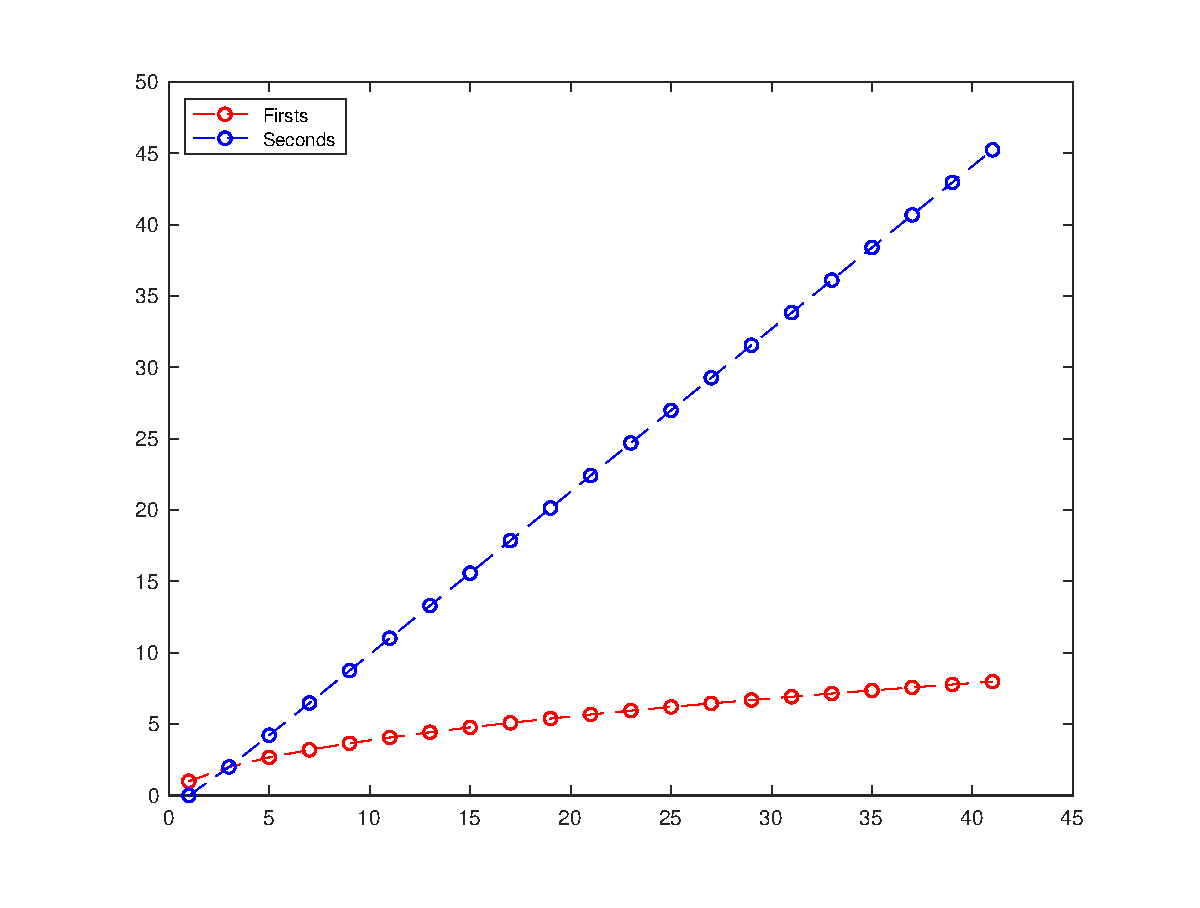
\includegraphics[width=12cm]{secs.eps}}\caption{The first and second order terms of the magnitude of odd-dimensional Euclidean balls.}\label{fig:secs}
\end{figure}

As we can see, the second order term looks to be linear in the dimension (as the first order term turns out to be proportional to the square root of the dimension). In fact, the Convex Magnitude Conjecture (which was shown to be false in \cite{barcelo_magnitudes_2016} with the explicit computation of the magnitude function of the 5-dimensional Euclidean ball) suggests that the second order term would be just $m$. Let's see what we get when we actually simplify our expression above.

\subsubsection*{$\sigma = L$}

We show that in fact the values of $\sigma$ and $L$ above are equal. By abuse of notation, denote $\sigma$ to be the set of disjoint $(m+1)$-collections that we are considering when computing the number $\sigma$ above and similarly for $L$. We will show that there is a bijection of sets $f:\sigma \to L$ that preserves the product of the weights.

Let $\delta$ be a disjoint $(m+1)$-collection in $\sigma$. In general, $\delta$ will have its first flat step at $p_1$ and second flat step at $p_2$. In between the two flat steps there will be $q_1$ $M$'s followed by $p_2-p_1-q_1$ number of upside down $V$'s. We'll call the height at which this first upside down $V$ path appears to be $v$. Then we define $f(\delta)$ to be a disjoint $(m+1)$-collection in $L$ where we take $\delta$ and replace the upside down $V$ path at $v$ with a off-centred flat step path and all the paths from $v+1$ up to $p_2$ are replaced with asymmetric $M$'s. If $\delta$ had no upside down $V$'s in between the first two flat steps, then just replace the second flat step with an off-centred flat step. Clearly $f(\delta)$ is a unique disjoint $(m+1)$-collection in $L$ and this defines a well-defined function of sets from $\sigma$ to $L$. We can see that $f$ preserves the product of the weights on $\delta$: each upside down $V$ path starting at a height of say, $h$ had product of weights $\frac{(2h-1)!}{(h-1)!}$ and this path was replaced by an asymmetric $M$ path with product of weights $\frac{(2h-2)!}{(h-1)!}$ but on the asymmetric $M$ path of height $h+1$ we have an extra factor of $(2(h+1)-3) = (2h+2-3) = (2h-1)$ so in total we also have product of weights $\frac{(2h-1)!}{(h-1)!}$. Note that this also applies to the flat step we introduced at height $v$: it had product of weights $\frac{(2v-2)!}{(v-1)!}$ but the asymmetric $M$ just above it gives an extra factor of $(2v-1)$ so we're fine. Finally the flat step at $p_2$ in $\delta$ had product of weights $\frac{(2p_2-2)!}{(p_2-1)}$ which is the same as the product of the weights in the asymmetric $M$ we introduced at $p_2$. So we see that $f$ preserves weighting.

Now we define a function $g:L\to\sigma$. Let $\delta$ instead be a disjoint $(m+1)$-collection in $L$. The collection $\delta$ has a second off-centred flat step at height $p_2$ with $q_1$ number of asymmetric $M$'s above it. Then we define $g(\delta)$ to be the disjoint $(m+1)$-collection where we replace the second flat step at $p_2$ and all the asymmetric $M$'s above it with upside down $V$'s except for the last one, which we turn into a centred flat step (ie. at height $p_2+q_1$. The paths above $p_2+q_1$ will be either upside down $V$'s or $M$'s and so this gives us a disjoint $(m+1)$-collection in $\sigma$. Clearly, $g,f$ are inverse to each other, giving us a bijection $\sigma\to L$. Since $f$ preserves products of weights, this also gives us that $\sigma = L$ as values.

\subsubsection*{$\sigma$ Term}

So by above, we have
\begin{equation*}
\frac{N''-d!D''}{N} = \frac{3\sigma}{N}
\end{equation*}

The denominator $N$ is given by
\begin{equation*}
N = \sum\limits_{\sigma \in X^0_{m+1}}\prod\limits_{\tau\in\sigma}\delta_2(\tau) = \prod\limits_{\tau \in X^{m+1}_\text{roof}}\delta_2(\tau) = \prod\limits_{k=0}^{m+1}\frac{(2k-1)!}{(k-1)!}
\end{equation*}

Earlier we had split $\sigma$ into four smaller sums based on which case they fell into. Consider a disjoint $(m+1)$-collection in the first case, that is, we fix $p_1 = 1$, $2\leq p_2\leq m+1$, $0\leq q_1\leq p_2 - 2$, $0\leq q_2 \leq m+1-p_2$. Then we have
\begin{align*}
\frac{\sigma'}{N} &= \frac{\left(\prod\limits_{k=2}^{q_1+2}(2k-2)!(2k-2)\right)\left(\prod\limits_{k=q_1+2}^{p_2-1}(2k-1)!\right)(2p_2-2)!\left(\prod\limits_{k=p_2+1}^{p_2+q_2}(2k-2)!(2k-2)\right)\left(\prod\limits_{k=p_2+q_2+1}^{m+1}(2k-1)!\right)}{\left(\prod\limits_{k=0}^{m+1}(2k-1)!\right)} \\
&= \frac{\left(\prod\limits_{k=2}^{q_1+2}(2k-2)!(2k-2)\right)(2p_2-2)!\left(\prod\limits_{k=p_2+1}^{p_2+q_2}(2k-2)!(2k-2)\right)}{\left(\prod\limits_{k=2}^{q_1+2}(2k-1)!\right)\left(\prod\limits_{k=p_2}^{p_2+q_2}(2k-1)!\right)} \\
&= \frac{1}{2p_2-1}\left(\prod\limits_{k=2}^{q_1+2}\frac{(2k-2)}{(2k-1)}\right)\left(\prod\limits_{k=p_2+1}^{p_2+q_2}\frac{(2k-2)}{(2k-1)}\right)
\end{align*}

So for the first case, we have
\begin{equation*}
\frac{\sigma_1}{N} = \sum\limits_{\substack{2\leq p_2\leq m+1 \\ 0\leq q_1 \leq p_2-2 \\ 0\leq q_2 \leq m+1-p_2}}\frac{1}{2p_2-1}\left(\prod\limits_{k=2}^{q_1+2}\frac{(2k-2)}{(2k-1)}\right)\left(\prod\limits_{k=p_2+1}^{p_2+q_2}\frac{(2k-2)}{(2k-1)}\right)
\end{equation*}

We similarly find expressions for the other three smaller sums.

Consider a disjoint $(m+1)$-collection in the second case, that is, we fix $2\leq p_1\leq m-1$,$p_2=m$,$0\leq q_1\leq m-p_1-1$, $q_2 = 1$. Then we have
\begin{equation*}
\frac{\sigma'}{N} = \frac{1}{2p_1-1}\left(\prod\limits_{k=p_1+1}^{p_1+q_1}\frac{(2k-2)}{(2k-1)}\right)\left(\frac{2m}{(2m-1)(2m+1)}\right)
\end{equation*}
and for the whole second case, we have
\begin{equation*}
\frac{\sigma_2}{N} = \sum\limits_{\substack{2\leq p_1\leq m-1 \\ 0\leq q_1\leq m-p_1-1}}\frac{1}{2p_1-1}\left(\prod\limits_{k=p_1+1}^{p_1+q_1}\frac{(2k-2)}{(2k-1)}\right)\left(\frac{2m}{(2m-1)(2m+1)}\right)
\end{equation*}

Consider a disjoint $(m+1)$-collection in the third case. Then we have
\begin{equation*}
\frac{\sigma'}{N} = \frac{1}{2p_1-1}\left(\prod\limits_{k=p_1+1}^{p_1+q_1}\frac{(2k-2)}{(2k-1)}\right)\left(\frac{1}{2m+1}\right)
\end{equation*}
and for the whole third case, we have
\begin{equation*}
\frac{\sigma_3}{N} = \sum\limits_{\substack{2\leq p_1\leq m \\ 0\leq q_1\leq m-p_1}}\frac{1}{2p_1-1}\left(\prod\limits_{k=p_1+1}^{p_1+q_1}\frac{(2k-2)}{(2k-1)}\right)\left(\frac{1}{2m+1}\right)
\end{equation*}

Consider a disjoint $(m+1)$-collection in the fourth case. Then we have
\begin{equation*}
\frac{\sigma'}{N} = \frac{1}{2p_1-1}\left(\prod\limits_{k=p_1+1}^{p_1+q_1}\frac{(2k-2)}{(2k-1)}\right)\frac{1}{2p_2-1}\left(\prod\limits_{k=p_2+1}^{m+1}\frac{(2k-2)}{(2k-1)}\right)
\end{equation*}
and for the whole fourth case, we have
\begin{equation*}
\frac{\sigma_4}{N} = \sum\limits_{\substack{2\leq p_1\leq m \\ p_1+1\leq p_2 \leq m-1 \\ 0\leq q_1\leq p_2-p_1-1 }}\frac{1}{2p_1-1}\left(\prod\limits_{k=p_1+1}^{p_1+q_1}\frac{(2k-2)}{(2k-1)}\right)\frac{1}{2p_2-1}\left(\prod\limits_{k=p_2+1}^{m+1}\frac{(2k-2)}{(2k-1)}\right)
\end{equation*}

\subsubsection*{Putting It All Together}

So all together we have
\begin{align*}
&\frac{d^2}{dt^2}\text{Mag}(tB_2^d)\big\vert_{t=0} = \\
&6\sum\limits_{\substack{2\leq p_2\leq m+1 \\ 0\leq q_1 \leq p_2-2 \\ 0\leq q_2 \leq m+1-p_2}}\frac{1}{2p_2-1}\left(\prod\limits_{k=2}^{q_1+2}\frac{(2k-2)}{(2k-1)}\right)\left(\prod\limits_{k=p_2+1}^{p_2+q_2}\frac{(2k-2)}{(2k-1)}\right) + \\
&6\sum\limits_{\substack{2\leq p_1\leq m-1 \\ 0\leq q_1\leq m-p_1-1}}\frac{1}{2p_1-1}\left(\prod\limits_{k=p_1+1}^{p_1+q_1}\frac{(2k-2)}{(2k-1)}\right)\left(\frac{2m}{(2m-1)(2m+1)}\right) + \\
&6\sum\limits_{\substack{2\leq p_1\leq m \\ 0\leq q_1\leq m-p_1}}\frac{1}{2p_1-1}\left(\prod\limits_{k=p_1+1}^{p_1+q_1}\frac{(2k-2)}{(2k-1)}\right)\left(\frac{1}{2m+1}\right) + \\
&6\sum\limits_{\substack{2\leq p_1\leq m \\ p_1+1\leq p_2 \leq m-1 \\ 0\leq q_1\leq p_2-p_1-1 }}\frac{1}{2p_1-1}\left(\prod\limits_{k=p_1+1}^{p_1+q_1}\frac{(2k-2)}{(2k-1)}\right)\frac{1}{2p_2-1}\left(\prod\limits_{k=p_2+1}^{m+1}\frac{(2k-2)}{(2k-1)}\right) - \\
&V_{1}\sum\limits_{\substack{1\leq p \leq m-1 \\ 0 \leq q \leq m - 1 - p}}\frac{1}{2p+1}\prod\limits_{k=p+1}^{p+q}\left(\frac{2k}{2k+1}\right)
\end{align*}

\pagebreak

\subsubsection*{Things to look at.}
\begin{enumerate}
\item Try to combine e+v and lemma 6.38 approach.
\item Try to apply negative type assumption to eigenvalue approach.
\item See what we can say about eigenvalues of matrices of negative type.
\end{enumerate}

\subsection*{Bounding the magnitude of a space of negative type by its cardinality.}

\subsubsection*{Eigenvalues}

Note that for a finite positive definite metric space
\begin{equation*}
\#A = \vert I_A \vert = \sup\limits_{v \neq 0}\frac{\left(\sum v(a)\right)^2}{v^\star I_A v} = \sup\limits_{v\neq0}\frac{\left(\sum v(a)\right)^2}{\Vert v \Vert^2}
\end{equation*}

We want to see if
\begin{equation*}
\vert tA \vert = \sup\limits_{v\neq0}\frac{\left(\sum v(a)\right)^2}{v^\star Z_{tA}v}\leq \vert I_A \vert
\end{equation*}

or equivalently if
\begin{equation*}
v^\star Z_{tA} v \geq \Vert v \Vert^2
\end{equation*}

Now since $Z_{tA}$ is positive definite, we can factorize $Z_{tA} = B^\star B$ where $B$ is Hermitian. So we have
\begin{equation*}
v^\star Z_{tA} v = v^\star B^\star B v = \langle Bv, Bv \rangle = \Vert Bv \Vert^2
\end{equation*}

so equivalently we have
\begin{equation*}
\Vert Bv \Vert^2 \geq \Vert v \Vert^2
\end{equation*}

Now by the Spectral decomposition, we have
\begin{equation*}
\Vert Bv \Vert^2 = \Vert U \Lambda U^\star v \Vert^2 = \Vert \Lambda U^\star v \Vert^2 = \sum\limits_{a \in tA} \vert \lambda_a y_a \vert^2 \quad \text{where $y = U^\star v$}
\end{equation*}

So the question is whether
\begin{equation*}
\sum\limits_{a\in tA} \vert \lambda_a y_a \vert^2 \geq \sum\limits_{a \in tA} \vert v_a \vert^2
\end{equation*}

So we want to understand the eigenvalues of the similarity matrix $Z_{tA}$. Some theorems and tools to look at are
\begin{enumerate}
\item Gersgorin Disc Theorem
\item Courant-Fischer Theorem
\item Work by Barcello-Carbery
\item Understand the matrix exponential more
\end{enumerate}

\subsubsection*{e + v decomposition}

Another approach that Professor Meckes suggested was in looking at the supremum expression for PD metric spaces to decompose things in terms of vectors $e + v$:

\begin{equation*}
\vert A \vert = \sup\limits_{x\neq0}\frac{\left(\sum x(a)\right)^2}{x^T Z x}
\end{equation*}

Now let $\#A = n$ and let $e$ be the all 1's vector. Then we can decompose $x = e + v$ where $e^T v = 0$. Then we have
\begin{equation*}
\sum x(a) = e^T x = e^T(e + v) = e^Te + e^Tv = e^Te = n
\end{equation*}

and so we have
\begin{align*}
\vert A \vert &= \sup\limits_{x\neq0}\frac{\left(\sum x(a)\right)^2}{x^T Z x} \\
&= \sup\limits_{\substack{v \in \mathbb{R}^A \\ e^Tv = 0}}\frac{n^2}{e^TZe + 2e^TZv + v^TZv} \quad\text{Symmetricity of $Z$}\\
&= \frac{n^2}{e^TZe + \inf\limits_{e^Tv = 0}(2e^TZv + v^TZv)} \\
&= \frac{n^2}{e^TZe + \inf\limits_{e^Tv=0}\left(-\frac{(e^TZv)^2}{v^TZv}\right)} \\
&= \frac{n^2}{e^TZe - \sup\limits_{e^Tv=0}\left(\frac{(e^TZv)^2}{v^TZv}\right)}
\end{align*}

So $\vert A \vert \leq n$ is equivalent to the condition that
\begin{equation*}
n \leq e^TZe - \sup\limits_{e^Tv = 0}\frac{(e^TZv)^2}{v^TZv}
\end{equation*}

which is equivalent to
\begin{equation*}
\sup\limits_{e^Tv=0}\frac{(e^TZv)^2}{v^TZv} \leq e^TZe - n = \sum\limits_{a,b}e^{-d(a,b)} - n = \sum\limits_{a\neq b} e^{-d{a,b)}}
\end{equation*}

which is equivalent to
\begin{equation*}
(e^TZv)^2 \leq (e^TZe - n)(v^TZv) \quad\text{whenever $e^Tv = 0$}
\end{equation*}

This looks kind of like a sort of Cauchy-Schwarz formula on the subspace $e^Tv=0$.

\subsubsection*{Lemma 6.38 Approach}
\begin{prop}[Lemma 6.38 of Zhan: Characterizing Negative Type]
Let $A$ be a real symmetric matrix of order $n$. Then the following are equivalent:
\begin{enumerate}
\item $A$ is conditionally positive semidefinite:
\begin{equation*}
x^TAx \geq 0 \quad\text{for all $x \in \Omega:=\{x \in \mathbb{R}^n : \sum x_i = 0\}$}
\end{equation*}
\item There is a $y \in \mathbb{R}^n$ such that the matrix $(a_{ij} - y_i - y_j)$ is positive semidefinite.
\item The Hadamard exponential $e^{\circ A}$ is infinitely divisible, that is, $e^{\circ \alpha A}$ is positive semidefinite for all $\alpha > 0$ (what we mean by negative type).
\end{enumerate}
\end{prop}

In our terms we have the matrix $\tilde{Z} = [-td(a,b)]_{a,b \in A}$. Then the following are equivalent:

\begin{enumerate}
\item $\tilde{Z}$ is conditionally positive semidefinite
\begin{equation*}
x^T\tilde{Z}x \geq 0 \quad\text{for all $x$ such that $\sum x_i = 0$}
\end{equation*}
\item there is a $y \in \mathbb{R}^n$ such that the matrix $(\tilde{Z}_{ij}-y_i-y_j) = (-td(i,j) - y_i - y_j)$ is positive semidefinite
\item $e^{\circ \tilde{Z}}$ is positive semidefinite for all $t > 0$ (i.e. $A$ is of negative type).
\end{enumerate}

For $x \in \mathbb{R}^n$, define
\begin{equation*}
\tilde{x} = x - n^{-1}(e^Tx)e = \begin{bmatrix} x_1 \\ \vdots \\ x_n \end{bmatrix} - \begin{bmatrix} \frac{\sum x_i}{n} \\ \vdots \\ \frac{\sum x_i}{n} \end{bmatrix}
\end{equation*}

Need to see that $\tilde{x} \in \Omega$ (Not sure here yet):
\begin{equation*}
\sum \tilde{x}_i = \sum \left(x_i - \frac{\sum x_i}{n}\right) = \sum\left(\frac{nx_i - \sum x_i}{n}\right)
\end{equation*}

The idea is to look at this vector $y$ and see if it gives us anything. Let $e$ be the all 1's vector. Define
\begin{equation*}
y = n^{-1}\tilde{Z}e - \frac{1}{2}n^{-2}(e^T\tilde{Z}e)e
\end{equation*}

Then since $\tilde{Z}$ is conditionally positive semidefinite, we have
\begin{equation*}
0 \leq \tilde{x}^T\tilde{Z}\tilde{x} = x^T(\tilde{Z} - ye^T - ey^T)x = x^T\tilde{Z}x - x^Tye^Tx - x^Tey^Tx
\end{equation*}
for all $x \in \mathbb{R}^n$.

If we substitute the expression we have for $y$ into the inequality above, we have
\begin{align*}
0 &\leq x^T\tilde{Z}x - x^Tye^Tx - x^Tey^Tx \\
&= x^T\tilde{Z}x - x^T\left(n^{-1}\tilde{Z}e - \frac{1}{2}n^{-2}(e^T\tilde{Z}e)e\right)e^Tx - x^Te\left(n^{-1}\tilde{Z}e-\frac{1}{2}n^{-2}(e^T\tilde{Z}e)e\right)^Tx
\end{align*}

Note that $e^Tx = x^Te = \sum x_i$. We'll denote this sum $X:=\sum x_i$. Also note that $e^T\tilde{Z}e = \sum\limits_{a,b\in A} -td(a,b)$. We'll denote this sum $K := \sum\limits_{a,b\in A} -td(a,b)$. Then the inequality above turns into
\begin{align*}
0 &\leq x^T\tilde{Z}x - x^Tye^Tx - x^Tey^Tx \\
&= x^T\tilde{Z}x - x^T\left(n^{-1}\tilde{Z}e - \frac{1}{2}n^{-2}(e^T\tilde{Z}e)e\right)e^Tx - x^Te\left(n^{-1}\tilde{Z}e-\frac{1}{2}n^{-2}(e^T\tilde{Z}e)e\right)^Tx \\
&= x^T\tilde{Z}x - x^T\left(n^{-1}\tilde{Z}e - \frac{1}{2}n^{-2}Ke\right)X - X\left(n^{-1}\tilde{Z}e-\frac{1}{2}n^{-2}Ke\right)^Tx
\end{align*}

Note also that the vector
\begin{equation*}
n^{-1}\tilde{Z}e = n^{-1}\begin{bmatrix}
-td(1,1) & \cdots & -td(1,n) \\
\vdots & \ddots & \vdots \\
-td(n,1) & \cdots & -td(n,n)
\end{bmatrix}\begin{bmatrix}
1 \\ \vdots \\ 1
\end{bmatrix} = n^{-1}\begin{bmatrix}
\sum_{a \in A} -td(a,1) \\ \vdots \\ \sum_{a \in A} -td(a,n)
\end{bmatrix}
\end{equation*}
which means something.

\nocite{*}
\bibliographystyle{alpha}
\bibliography{refs.bib}

\end{document}